%%%%%%%%%%%%%%%%%%%%%%%%%%%%%%%%%%%%%%%%%
% Style based on: The Legrand Orange Book - Version 1.4 (12/4/14)
%
% The original template has been downloaded from:
% http://www.LaTeXTemplates.com
%
% Original author:
% Mathias Legrand (legrand.mathias@gmail.com)
%
% License:
% CC BY-NC-SA 3.0 (http://creativecommons.org/licenses/by-nc-sa/3.0/)
%%%%%%%%%%%%%%%%%%%%%%%%%%%%%%%%%%%%%%%%%

%----------------------------------------------------------------------------------------
%	PACKAGES AND OTHER DOCUMENT CONFIGURATIONS
%----------------------------------------------------------------------------------------

\documentclass[11pt,fleqn,oneside,openany]{book} % Default font size and left-justified equations

\usepackage[top=3cm,bottom=3cm,left=3.2cm,right=3.2cm,headsep=10pt,a4paper]{geometry} % Page margins

\usepackage{xcolor} % Required for specifying colors by name
\definecolor{ocre}{RGB}{243,102,25} % Define the orange color used for highlighting throughout the book
\definecolor{brown}{RGB}{192,81,20} % Define the brown color used for highlighting of URLs throughout the book

% Font Settings
\usepackage{avant} % Use the Avantgarde font for headings
%\usepackage{times} % Use the Times font for headings
\usepackage{mathptmx} % Use the Adobe Times Roman as the default text font together with math symbols from the Sym­bol, Chancery and Com­puter Modern fonts

\usepackage{microtype} % Slightly tweak font spacing for aesthetics
\usepackage[utf8]{inputenc} % Required for including letters with accents
\usepackage[T1]{fontenc} % Use 8-bit encoding that has 256 glyphs

% Bibliography
%\usepackage[style=alphabetic,sorting=nyt,sortcites=true,autopunct=true,babel=hyphen,hyperref=true,abbreviate=false,backref=true,backend=biber]{biblatex}
%\addbibresource{bibliography.bib} % BibTeX bibliography file
%\defbibheading{bibempty}{}

% Index
%\usepackage{calc} % For simpler calculation - used for spacing the index letter headings correctly
%\usepackage{makeidx} % Required to make an index
%\makeindex % Tells LaTeX to create the files required for indexing

%----------------------------------------------------------------------------------------
%	VARIOUS REQUIRED PACKAGES
%----------------------------------------------------------------------------------------

\usepackage{titlesec} % Allows customization of titles

\usepackage{graphicx} % Required for including images
\graphicspath{{images/}} % Specifies the directory where images are stored

\usepackage{lipsum} % Inserts dummy text

\usepackage{tikz} % Required for drawing custom shapes

\usepackage[english]{babel} % English language/hyphenation

\usepackage{enumitem} % Customize lists
\setlist{nolistsep} % Reduce spacing between bullet points and numbered lists

\usepackage{booktabs} % Required for nicer horizontal rules in tables

\usepackage{eso-pic} % Required for specifying an image background in the title page

%----------------------------------------------------------------------------------------
%	MAIN TABLE OF CONTENTS
%----------------------------------------------------------------------------------------

\usepackage{titletoc} % Required for manipulating the table of contents

\contentsmargin{0cm} % Removes the default margin
% Chapter text styling
\titlecontents{chapter}[1.25cm] % Indentation
{\addvspace{15pt}\large\sffamily\bfseries} % Spacing and font options for chapters
{\color{ocre!60}\contentslabel[\Large\thecontentslabel]{1.25cm}\color{ocre}} % Chapter number
{}  
{\color{ocre!60}\normalsize\sffamily\bfseries\;\titlerule*[.5pc]{.}\;\thecontentspage} % Page number
% Section text styling
\titlecontents{section}[1.25cm] % Indentation
{\addvspace{5pt}\sffamily\bfseries} % Spacing and font options for sections
{\contentslabel[\thecontentslabel]{1.25cm}} % Section number
{}
{\sffamily\hfill\color{black}\thecontentspage} % Page number
[]
% Subsection text styling
\titlecontents{subsection}[1.25cm] % Indentation
{\addvspace{1pt}\sffamily\small} % Spacing and font options for subsections
{\contentslabel[\thecontentslabel]{1.25cm}} % Subsection number
{}
{\sffamily\;\titlerule*[.5pc]{.}\;\thecontentspage} % Page number
[] 

%----------------------------------------------------------------------------------------
%	MINI TABLE OF CONTENTS IN CHAPTER HEADS
%----------------------------------------------------------------------------------------

% Section text styling
\titlecontents{lsection}[0em] % Indendating
{\footnotesize\sffamily} % Font settings
{}
{}
{}

% Subsection text styling
\titlecontents{lsubsection}[.5em] % Indentation
{\normalfont\footnotesize\sffamily} % Font settings
{}
{}
{}
 
%----------------------------------------------------------------------------------------
%	PAGE HEADERS
%----------------------------------------------------------------------------------------

\usepackage{fancyhdr} % Required for header and footer configuration

\pagestyle{fancy}
\renewcommand{\chaptermark}[1]{\markboth{\sffamily\normalsize\bfseries\chaptername\ \thechapter.\ #1}{}} % Chapter text font settings
\renewcommand{\sectionmark}[1]{\markright{\sffamily\normalsize\thesection\hspace{5pt}#1}{}} % Section text font settings
\fancyhf{} \fancyhead[LE,RO]{\sffamily\normalsize\thepage} % Font setting for the page number in the header
\fancyhead[LO]{\rightmark} % Print the nearest section name on the left side of odd pages
\fancyhead[RE]{\leftmark} % Print the current chapter name on the right side of even pages
\renewcommand{\headrulewidth}{0.5pt} % Width of the rule under the header
\addtolength{\headheight}{2.5pt} % Increase the spacing around the header slightly
\renewcommand{\footrulewidth}{0pt} % Removes the rule in the footer
\fancypagestyle{plain}{\fancyhead{}\renewcommand{\headrulewidth}{0pt}} % Style for when a plain pagestyle is specified

% Removes the header from odd empty pages at the end of chapters
\makeatletter
\renewcommand{\cleardoublepage}{
\clearpage\ifodd\c@page\else
\hbox{}
\vspace*{\fill}
\thispagestyle{empty}
\newpage
\fi}

%----------------------------------------------------------------------------------------
%	THEOREM STYLES
%----------------------------------------------------------------------------------------

\usepackage{amsmath,amsfonts,amssymb,amsthm} % For math equations, theorems, symbols, etc

\newcommand{\intoo}[2]{\mathopen{]}#1\,;#2\mathclose{[}}
\newcommand{\ud}{\mathop{\mathrm{{}d}}\mathopen{}}
\newcommand{\intff}[2]{\mathopen{[}#1\,;#2\mathclose{]}}
\newtheorem{notation}{Notation}[chapter]

%%%%%%%%%%%%%%%%%%%%%%%%%%%%%%%%%%%%%%%%%%%%%%%%%%%%%%%%%%%%%%%%%%%%%%%%%%%
%%%%%%%%%%%%%%%%%%%% dedicated to boxed/framed environements %%%%%%%%%%%%%%
%%%%%%%%%%%%%%%%%%%%%%%%%%%%%%%%%%%%%%%%%%%%%%%%%%%%%%%%%%%%%%%%%%%%%%%%%%%
\newtheoremstyle{ocrenumbox}% % Theorem style name
{0pt}% Space above
{0pt}% Space below
{\normalfont}% % Body font
{}% Indent amount
{\small\bf\sffamily\color{ocre}}% % Theorem head font
{\;}% Punctuation after theorem head
{0.25em}% Space after theorem head
{\small\sffamily\color{ocre}\thmname{#1}\nobreakspace\thmnumber{\@ifnotempty{#1}{}\@upn{#2}}% Theorem text (e.g. Theorem 2.1)
\thmnote{\nobreakspace\the\thm@notefont\sffamily\bfseries\color{black}---\nobreakspace#3.}} % Optional theorem note
\renewcommand{\qedsymbol}{$\blacksquare$}% Optional qed square

\newtheoremstyle{blacknumex}% Theorem style name
{5pt}% Space above
{5pt}% Space below
{\normalfont}% Body font
{} % Indent amount
{\small\bf\sffamily}% Theorem head font
{\;}% Punctuation after theorem head
{0.25em}% Space after theorem head
{\small\sffamily{\tiny\ensuremath{\blacksquare}}\nobreakspace\thmname{#1}\nobreakspace\thmnumber{\@ifnotempty{#1}{}\@upn{#2}}% Theorem text (e.g. Theorem 2.1)
\thmnote{\nobreakspace\the\thm@notefont\sffamily\bfseries---\nobreakspace#3.}}% Optional theorem note

\newtheoremstyle{blacknumbox} % Theorem style name
{0pt}% Space above
{0pt}% Space below
{\normalfont}% Body font
{}% Indent amount
{\small\bf\sffamily}% Theorem head font
{\;}% Punctuation after theorem head
{0.25em}% Space after theorem head
{\small\sffamily\thmname{#1}\nobreakspace\thmnumber{\@ifnotempty{#1}{}\@upn{#2}}% Theorem text (e.g. Theorem 2.1)
\thmnote{\nobreakspace\the\thm@notefont\sffamily\bfseries---\nobreakspace#3.}}% Optional theorem note

%%%%%%%%%%%%%%%%%%%%%%%%%%%%%%%%%%%%%%%%%%%%%%%%%%%%%%%%%%%%%%%%%%%%%%%%%%%
%%%%%%%%%%%%% dedicated to non-boxed/non-framed environements %%%%%%%%%%%%%
%%%%%%%%%%%%%%%%%%%%%%%%%%%%%%%%%%%%%%%%%%%%%%%%%%%%%%%%%%%%%%%%%%%%%%%%%%%
\newtheoremstyle{ocrenum}% % Theorem style name
{5pt}% Space above
{5pt}% Space below
{\normalfont}% % Body font
{}% Indent amount
{\small\bf\sffamily\color{ocre}}% % Theorem head font
{\;}% Punctuation after theorem head
{0.25em}% Space after theorem head
{\small\sffamily\color{ocre}\thmname{#1}\nobreakspace\thmnumber{\@ifnotempty{#1}{}\@upn{#2}}% Theorem text (e.g. Theorem 2.1)
\thmnote{\nobreakspace\the\thm@notefont\sffamily\bfseries\color{black}---\nobreakspace#3.}} % Optional theorem note
\renewcommand{\qedsymbol}{$\blacksquare$}% Optional qed square
\makeatother

% Defines the theorem text style for each type of theorem to one of the three styles above
\newcounter{dummy} 
\numberwithin{dummy}{section}
\theoremstyle{ocrenumbox}
\newtheorem{theoremeT}[dummy]{Theorem}
\newtheorem{problem}{Problem}[chapter]
\newtheorem{exerciseT}{Exercise}[chapter]
\theoremstyle{blacknumex}
\newtheorem{exampleT}{Example}[chapter]
\theoremstyle{blacknumbox}
\newtheorem{vocabulary}{Vocabulary}[chapter]
\newtheorem{definitionT}{Definition}[section]
\newtheorem{corollaryT}[dummy]{Corollary}
\theoremstyle{ocrenum}
\newtheorem{proposition}[dummy]{Proposition}

%----------------------------------------------------------------------------------------
%	DEFINITION OF COLORED BOXES
%----------------------------------------------------------------------------------------

\RequirePackage[framemethod=default]{mdframed} % Required for creating the theorem, definition, exercise and corollary boxes

% Theorem box
\newmdenv[skipabove=7pt,
skipbelow=7pt,
backgroundcolor=black!5,
linecolor=ocre,
innerleftmargin=5pt,
innerrightmargin=5pt,
innertopmargin=5pt,
leftmargin=0cm,
rightmargin=0cm,
innerbottommargin=5pt]{tBox}

% Exercise box	  
\newmdenv[skipabove=7pt,
skipbelow=7pt,
rightline=false,
leftline=true,
topline=false,
bottomline=false,
backgroundcolor=ocre!10,
linecolor=ocre,
innerleftmargin=5pt,
innerrightmargin=5pt,
innertopmargin=5pt,
innerbottommargin=5pt,
leftmargin=0cm,
rightmargin=0cm,
linewidth=4pt]{eBox}	

% Definition box
\newmdenv[skipabove=7pt,
skipbelow=7pt,
rightline=false,
leftline=true,
topline=false,
bottomline=false,
linecolor=ocre,
innerleftmargin=5pt,
innerrightmargin=5pt,
innertopmargin=0pt,
leftmargin=0cm,
rightmargin=0cm,
linewidth=4pt,
innerbottommargin=0pt]{dBox}	

% Corollary box
\newmdenv[skipabove=7pt,
skipbelow=7pt,
rightline=false,
leftline=true,
topline=false,
bottomline=false,
linecolor=gray,
backgroundcolor=black!5,
innerleftmargin=5pt,
innerrightmargin=5pt,
innertopmargin=5pt,
leftmargin=0cm,
rightmargin=0cm,
linewidth=4pt,
innerbottommargin=5pt]{cBox}

% Creates an environment for each type of theorem and assigns it a theorem text style from the "Theorem Styles" section above and a colored box from above
\newenvironment{theorem}{\begin{tBox}\begin{theoremeT}}{\end{theoremeT}\end{tBox}}
\newenvironment{exercise}{\begin{eBox}\begin{exerciseT}}{\hfill{\color{ocre}\tiny\ensuremath{\blacksquare}}\end{exerciseT}\end{eBox}}
\newenvironment{definition}{\begin{dBox}\begin{definitionT}}{\end{definitionT}\end{dBox}}	
\newenvironment{example}{\begin{exampleT}}{\hfill{\tiny\ensuremath{\blacksquare}}\end{exampleT}}		
\newenvironment{corollary}{\begin{cBox}\begin{corollaryT}}{\end{corollaryT}\end{cBox}}	

%----------------------------------------------------------------------------------------
%	REMARK ENVIRONMENT
%----------------------------------------------------------------------------------------

\newenvironment{remark}{\par\vspace{10pt}\small % Vertical white space above the remark and smaller font size
\begin{list}{}{
\leftmargin=35pt % Indentation on the left
\rightmargin=25pt}\item\ignorespaces % Indentation on the right
\makebox[-2.5pt]{\begin{tikzpicture}[overlay]
\node[draw=ocre!60,line width=1pt,circle,fill=ocre!25,font=\sffamily\bfseries,inner sep=2pt,outer sep=0pt] at (-15pt,0pt){\textcolor{ocre}{R}};\end{tikzpicture}} % Orange R in a circle
\advance\baselineskip -1pt}{\end{list}\vskip5pt} % Tighter line spacing and white space after remark

%----------------------------------------------------------------------------------------
%	SECTION NUMBERING IN THE MARGIN
%----------------------------------------------------------------------------------------

\makeatletter
\renewcommand{\@seccntformat}[1]{\llap{\textcolor{ocre}{\csname the#1\endcsname}\hspace{1em}}}                    
\renewcommand{\section}{\@startsection{section}{1}{\z@}
{-4ex \@plus -1ex \@minus -.4ex}
{1ex \@plus.2ex }
{\normalfont\large\sffamily\bfseries}}
\renewcommand{\subsection}{\@startsection {subsection}{2}{\z@}
{-3ex \@plus -0.1ex \@minus -.4ex}
{0.5ex \@plus.2ex }
{\normalfont\sffamily\bfseries}}
\renewcommand{\subsubsection}{\@startsection {subsubsection}{3}{\z@}
{-2ex \@plus -0.1ex \@minus -.2ex}
{.2ex \@plus.2ex }
{\normalfont\small\sffamily\bfseries}}                        
\renewcommand\paragraph{\@startsection{paragraph}{4}{\z@}
{-2ex \@plus-.2ex \@minus .2ex}
{.1ex}
{\normalfont\small\sffamily\bfseries}}

%----------------------------------------------------------------------------------------
%	HYPERLINKS IN THE DOCUMENTS
%----------------------------------------------------------------------------------------

% For an unclear reason, the package should be loaded now and not later
\usepackage{hyperref}
\hypersetup{hidelinks,backref=true,pagebackref=true,hyperindex=false,
colorlinks=true,breaklinks=true,urlcolor=ocre,linkcolor=black,
bookmarks=true,bookmarksopen=false,pdftitle={Title},pdfauthor={Author}}

%----------------------------------------------------------------------------------------
%	CHAPTER HEADINGS
%----------------------------------------------------------------------------------------

% The set-up below should be (sadly) manually adapted to the overall margin page septup controlled by the geometry package loaded in the main.tex document. It is possible to implement below the dimensions used in the goemetry package (top,bottom,left,right)... TO BE DONE

\newcommand{\thechapterimage}{}
\newcommand{\chapterimage}[1]{\renewcommand{\thechapterimage}{#1}}

% Numbered chapters with mini tableofcontents
\def\thechapter{\arabic{chapter}}
\def\@makechapterhead#1{
\thispagestyle{empty}
{\centering \normalfont\sffamily
\ifnum \c@secnumdepth >\m@ne
\if@mainmatter
\startcontents
\begin{tikzpicture}[remember picture,overlay]
\node at (current page.north west)
{\begin{tikzpicture}[remember picture,overlay]
\node[anchor=north west,inner sep=0pt] at (0,0) {\includegraphics[width=\paperwidth]{\thechapterimage}};
%%%%%%%%%%%%%%%%%%%%%%%%%%%%%%%%%%%%%%%%%%%%%%%%%%%%%%%%%%%%%%%%%%%%%%%%%%%%%%%%%%%%%
% Commenting the 3 lines below removes the small contents box in the chapter heading
\fill[color=ocre!10!white,opacity=.6] (1cm,0) rectangle (8cm,-7cm);
\node[anchor=north west] at (1.1cm,.35cm) {\parbox[t][8cm][t]{6.5cm}{\huge\bfseries\flushleft \vspace*{9pt} \printcontents{l}{1}{\setcounter{tocdepth}{2}}}};
\draw[anchor=west] (5cm,-9cm) node [rounded corners=20pt,fill=ocre!10!white,text opacity=1,draw=ocre,draw opacity=1,line width=1.5pt,fill opacity=.6,inner sep=12pt]{\huge\sffamily\bfseries\textcolor{black}{\thechapter. #1\strut\makebox[22cm]{}}};
%%%%%%%%%%%%%%%%%%%%%%%%%%%%%%%%%%%%%%%%%%%%%%%%%%%%%%%%%%%%%%%%%%%%%%%%%%%%%%%%%%%%%
\end{tikzpicture}};
\end{tikzpicture}}
\par\vspace*{230\p@}
\fi
\fi}

% Unnumbered chapters without mini tableofcontents (could be added though) 
\def\@makeschapterhead#1{
\thispagestyle{empty}
{\centering \normalfont\sffamily
\ifnum \c@secnumdepth >\m@ne
\if@mainmatter
\begin{tikzpicture}[remember picture,overlay]
\node at (current page.north west)
{\begin{tikzpicture}[remember picture,overlay]
\node[anchor=north west,inner sep=0pt] at (0,0) {\includegraphics[width=\paperwidth]{\thechapterimage}};
\draw[anchor=west] (5cm,-9cm) node [rounded corners=20pt,fill=ocre!10!white,fill opacity=.6,inner sep=12pt,text opacity=1,draw=ocre,draw opacity=1,line width=1.5pt]{\huge\sffamily\bfseries\textcolor{black}{#1\strut\makebox[22cm]{}}};
\end{tikzpicture}};
\end{tikzpicture}}
\par\vspace*{230\p@}
\fi
\fi
}
\makeatother
 % Insert the structure.tex file which contains the majority of the structure behind the template

%----------------------------------------------------------------------------------------
%	EXTRA PACKAGES AND SETTINGS
%----------------------------------------------------------------------------------------

% Include package for fancy verbatim environment.
\usepackage{fancyvrb}

% Define color of verbatim fonts.
\renewcommand{\FancyVerbFormatLine}[1]{\textcolor{ocre}{#1}}

% Redefine verbatim environment.
\DefineVerbatimEnvironment{verbatim}{Verbatim}{frame=leftline, framerule=4pt, framesep=10pt, rulecolor=\color{ocre}}

% Define symbols for itemized lists
\renewcommand{\labelitemi}{\textcolor{ocre}{$\blacktriangleright$}}
\renewcommand{\labelitemii}{\textcolor{ocre}{$\vartriangleright$}}
\renewcommand{\labelitemiii}{\textcolor{ocre}{$\scriptstyle\vartriangleright$}}

% For itemization with cirecled numbers and other fancy stuff ...
%\usepackage{pifont}

% For visualization of keystrokes.
\usepackage{menukeys} 

% The following is in general not recommended, but package 'parskip' does not work properly with this style ...
\setlength{\parindent}{0pt}
\setlength{\parskip}{4pt}

% Use date and time to construct a version number for the document
\usepackage{datetime}
\newcommand{\versionsep}{-}
\renewcommand{\dateseparator}{\versionsep}
\renewcommand{\timeseparator}{\versionsep}

% Declare allowed graphics extensions
\DeclareGraphicsExtensions{.pdf,.png,.jpg}

% Custom declarations.
\usepackage{xspace} % Defines a 'smart space' (not present before punctuation)
\newcommand{\fmipp}{FMI++\xspace}
\newcommand{\trnsys}{TRNSYS\xspace}
\newcommand{\boost}{Boost\xspace}
\newcommand{\dymola}{Dymola\xspace}
\newcommand{\python}{Python\xspace}

\newcommand{\type}{Type6139\xspace}
\newcommand{\typea}{Type6139a\xspace}
\newcommand{\typeb}{Type6139b\xspace}


\begin{document}

%----------------------------------------------------------------------------------------
%	TITLE PAGE
%----------------------------------------------------------------------------------------

\begingroup
\thispagestyle{empty}
\AddToShipoutPicture*{\put(6,5){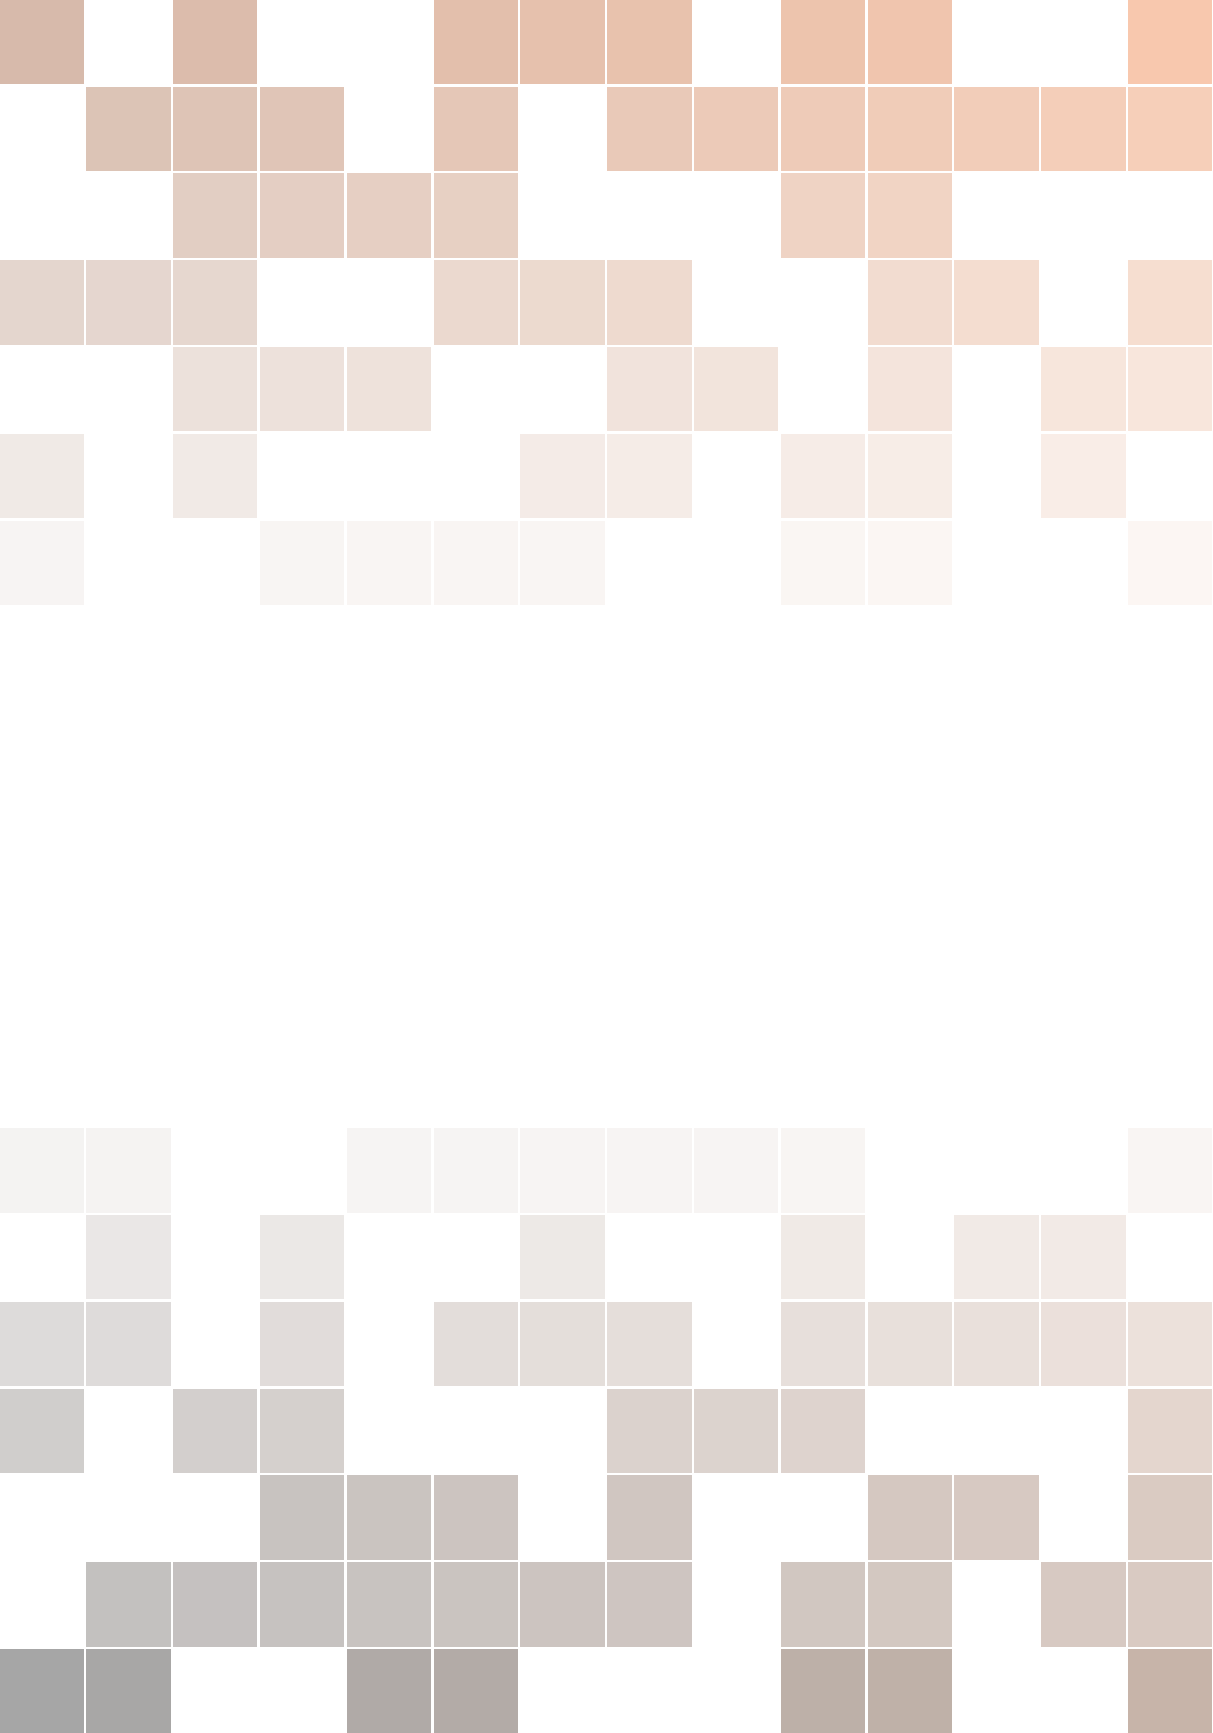
\includegraphics[scale=1]{background_main}}} % Image background
\centering
\vspace*{9.35cm}
\par\normalfont\fontsize{29}{30}\sffamily\selectfont
The \fmipp \trnsys FMU Export Utility\par % Book title
\vspace*{0.5cm}
{\huge Documentation}\\[5pt]
{\normalsize v\yyyymmdddate\today\versionsep\currenttime}\par % Subtitle
\endgroup

%----------------------------------------------------------------------------------------
%	COPYRIGHT PAGE
%----------------------------------------------------------------------------------------

\newpage
~\vfill
\thispagestyle{empty}

\noindent \trnsys~\textregistered~is a registered trademark of Solar Energy Laboratory, University of Wisconsin-Madison.

\noindent Dymola~\textregistered~is a registered trademark of Dassault Syst\`emes AB.

\noindent Other product or brand names are trademarks or registered trademarks of their respective holders.

\vspace*{2cm}

\noindent Copyright \copyright\ 2015-2016 AIT Austrian Institute of Technology\\ % Copyright notice

%\noindent \textsc{Published by Publisher}\\ % Publisher

\noindent Available at: \url{http://trnsys-fmu.sourceforge.net/}\\ % URL

\noindent Licensed under the Creative Commons Attribution-NonCommercial 3.0 Unported License (the ``License''). You may not use this file except in compliance with the License. You may obtain a copy of the License at \url{http://creativecommons.org/licenses/by-nc/3.0}. Unless required by applicable law or agreed to in writing, software distributed under the License is distributed on an \textsc{``as is'' basis, without warranties or conditions of any kind}, either express or implied. See the License for the specific language governing permissions and limitations under the License.\\ % License information

%\noindent \textit{First printing, March 2013} % Printing/edition date

%----------------------------------------------------------------------------------------
%	TABLE OF CONTENTS
%----------------------------------------------------------------------------------------

\chapterimage{toc_head.pdf} % Table of contents heading image

\pagestyle{empty} % No headers

\tableofcontents % Print the table of contents itself

%\cleardoublepage % Forces the first chapter to start on an odd page so it's on the right

\pagestyle{fancy} % Print headers again

%----------------------------------------------------------------------------------------
%	CHAPTERS
%----------------------------------------------------------------------------------------

\chapterimage{chapter_head.pdf} % Chapter heading image

\chapter{Introduction}


\section{About}

The \href{http://trnsys-fmu.sourceforge.net}{\fmipp \trnsys FMU Export Utility} is a stand-alone tool for exporting FMUs for Co-Simulation (\href{https://www.fmi-standard.org/}{FMI Version~1.0}) from \href{http://www.trnsys.com/}{\trnsys} models. It is open-source (see license in Section~\ref{trnsys_fmu_license}) and \href{http://trnsys-fmu.sourceforge.net}{freely available}. It is based on code from the \href{http://fmipp.sourceforge.net}{FMI++ library} (see license in Section~\ref{fmipp_license}) and the \href{http://www.boost.org/}{Boost C++ libraries} (see license in Section~\ref{boost_license}).

The \fmipp \trnsys FMU Export Utility provides the following functionality:
\begin{itemize}
  \item A dedicated \trnsys block called \type that may be included in \trnsys models in order to make them available to external application via an FMI-compliant simulation interface. This interface allows external applications to retrieve/send data from/to a \trnsys model at runtime. The name of \type comes from the position of the letters F, M and I in the alphabet---6, 13 and 9 respectively.
  \item A graphical user interface (or alternatively a \href{https://www.python.org/}{\python} script) that creates FMUs from \trnsys models, including the XML model description and shared libraries. Additional files (e.g., weather files) and start values for exported variables can be specified.
\end{itemize}

\section{Basic functionality}

The \fmipp library introduces the concept of \emph{front end}, \emph{back end} and \emph{adapter} for developing FMI interfaces for a wide variety of tools.\footnote{For more detailed information, please refer to this publication: \href{https://modelica.org/events/modelica2017/proceedings/html/submissions/ecp17132321_WidlMuller.pdf}{E.~Widl and W.~M\"uller, "\textit{Generic FMI-compliant Simulation Tool Coupling}", Proc. of the 12th International Modelica Conference, Prague, Czech Republic, 2017}} This concept has been adopted to implement the \fmipp \trnsys FMU Export Utility:
\begin{itemize}
  \item The front end implements the \emph{fmiComponent}, which is used by an external application---the master algorithm---to interact with \trnsys. Via this front end the master algorithm is able to control the simulation execution (start, stop, make step) and can retrieve/send data from/to \trnsys at runtime.
  \item The back end is a generic gateway between \trnsys and the front end that enables runtime control and data exchange. This connection is established via shared memory access.
  \item The adapter is a dedicated component in the simulation tool that utilizes the back end. In the case of \trnsys the adapter is called \type.
\end{itemize}
Figure~\ref{fig:schematics} gives a schematic overview of how this concept is applied to \trnsys. The master algorithm accesses \trnsys via the front end, which is connected to the back end via shared memory access. The back end is used by \type, which is part of the \trnsys model.

\begin{figure}[h!]
\centering{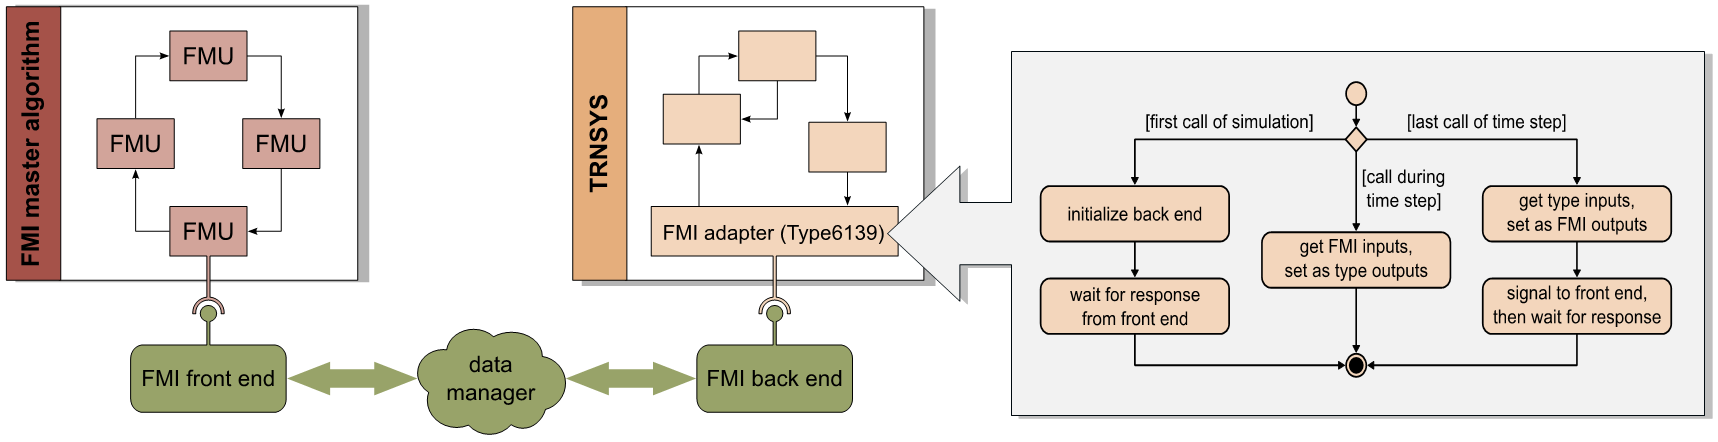
\includegraphics[width=\textwidth]{trnsys_export_schematics}}
\caption{Schematics of \fmipp \trnsys FMU export.}
\label{fig:schematics}
\end{figure}

\chapter{Installation and Configuration}

\section{Software requirements}

The \fmipp \trnsys FMU Export Utility is intended to run on Windows~7~(32-bit).

The following applications need to be installed prior to installing the \fmipp \trnsys FMU Export Utility:
\begin{itemize}

  \item \href{http://www.trnsys.com/}{\trnsys~17}

  \item For creating FMUs from command line \href{https://www.python.org/}{\python} (tested with \python~3.5) is required.

  \item For compiling FMU according to FMI version 1.0 a version of Microsoft Visual Studio Express 2013 for Windows Desktop has to be installed.
\end{itemize}

\textbf{Note}: For generating FMUs with the help of the graphical user interface \python is not required.

\textbf{Note}: For generating FMUs according to FMI version 2.0 (default) Microsoft Visual Studio Express 2013 for Windows Desktop is not required!


\section{Installation}
\label{sec:install}

To install the \fmipp \trnsys FMU Export Utility , proceed as follows:
\begin{itemize}

  \item Download the latest version as ZIP-file from the \href{http://sourceforge.net/projects/trnsys-fmu/files/latest/download}{download page}.

  \item Unzip the installation file into any sub directory (referred to as the \emph{installation directory}).

  \item Switch to the installation directory and start program \texttt{trnsys\_fmu\_install.exe} (double-click).
  This should bring up the window shown in Figure~\ref{fig:trnsys_fmu_install_gui}.

  \item Provide the path to the TRNSYS installation directory and press \textit{Start}.

\end{itemize}

After successful installation, \type is available in the \trnsys Simulation Studio. An additional directory called \emph{FMI} should be available in the toolbar on the right-hand side, containing the new \trnsys type (\emph{\typea} and \emph{\typeb}), see Figure~\ref{fig:simulation_studio_overview} for a snapshot.


\section{Installation using a Python script}
\label{sec:install_script}

Alternatively, the installation can be done by running a Python script.
This requires to execute \python from the command prompt window, please refer to the \href{https://docs.python.org/2/faq/windows.html}{\python~FAQ} in case you need assistance with this.
Open the command prompt window, change to the installation directory and execute the script \texttt{trnsys\_fmu\_install.py}:
\begin{verbatim}
python.exe trnsys_fmu_install.py <trnsys_install_dir>
\end{verbatim}
where \texttt{<trnsys\_install\_dir>} is the path to your local \trnsys installation directory (typically \texttt{C:\symbol{92}Trnsys17}).

\begin{figure}[h]
\centering{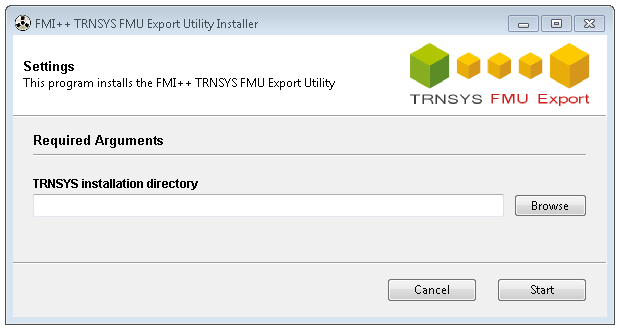
\includegraphics[width=0.98\textwidth]{trnsys_fmu_install_gui}}
\caption{View of the FMI++ TRNSYS FMU Export Utility installer.}
\label{fig:trnsys_fmu_install_gui}
\end{figure}

\begin{figure}[h]
\centering{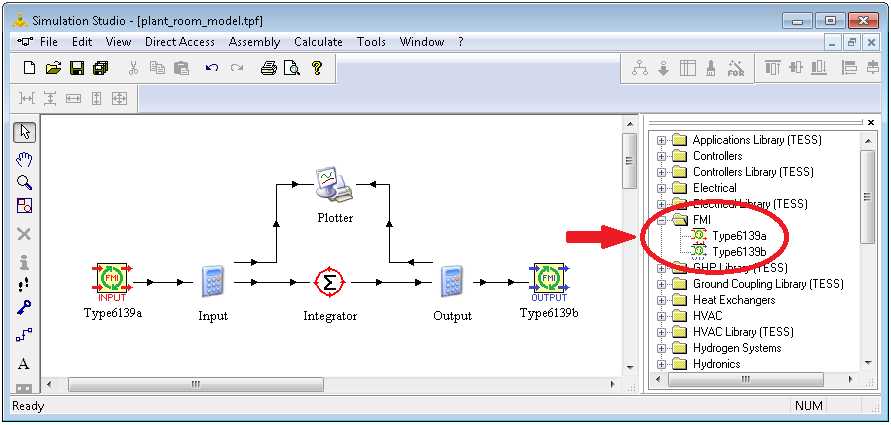
\includegraphics[width=\textwidth]{simulation_studio_overview}}
\caption{Simulation Studio with \type successfully installed.}
\label{fig:simulation_studio_overview}
\end{figure}


\chapter{Exporting \trnsys models as FMUs}

\section{Including \type in a \trnsys model}
\label{sec:export:model}

To export a \trnsys model as FMU for Co-Simulation, \type has to be properly included into the model.
\type comes in two variants:
\begin{itemize}
  \item \textbf{\typea}: \emph{Inputs to} the FMU (from the master algorithm) are this type's outputs.
  \item \textbf{\typeb}: This type's inputs are the \emph{outputs from} the FMU (to the master algorithm).
\end{itemize}
The inputs and outputs of the FMU are defined via the \emph{special cards tabs} of \typea and \typeb. In case the information in these tabs is missing (or incomplete), the resulting FMU will not work properly!

Figure~\ref{fig:trnsys_model} shows a screen shot from Simulation Studio with a simple \trnsys model that includes an instance of \typea and \typeb.

\begin{figure}[h]
\centering{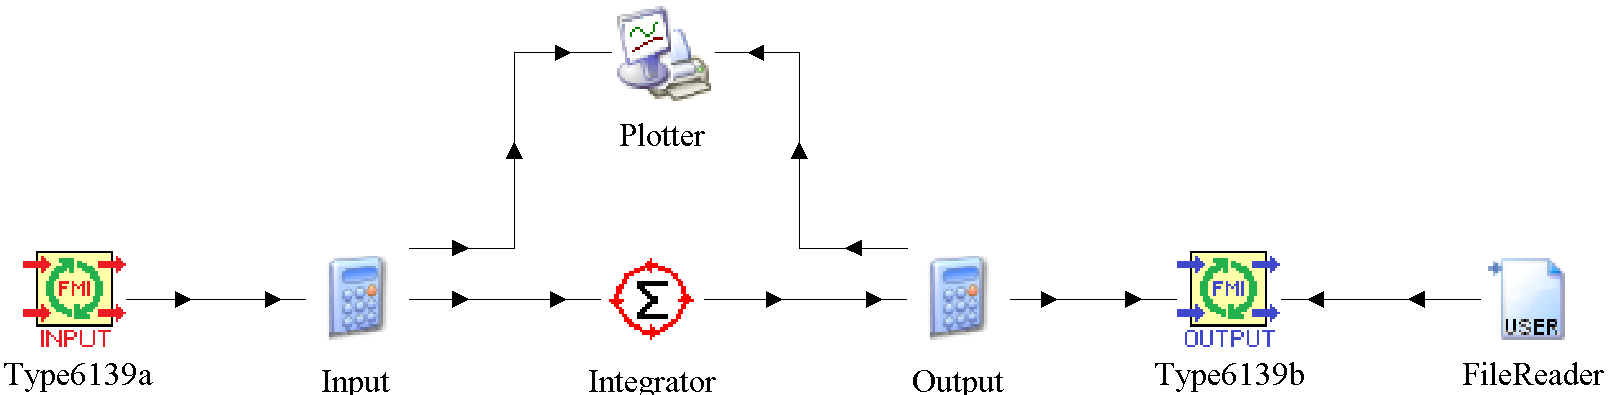
\includegraphics[width=0.95\textwidth]{trnsys_model}}
\caption{Example \trnsys model}
\label{fig:trnsys_model}
\end{figure}

\subsection{Configuring \typea}
With the help of Simulation Studio, configuration of \typea is simple:
\begin{itemize}
  \item Add the type to the model (via drag and drop from the toolbar on the right).
  \item Double-click the type icon to access its \emph{proforma}.
  There are 3 important tabs:
  \begin{itemize}
    \item \emph{Parameter tab}: Enter the number of FMU inputs, i.e., the number of inputs from the master algorithm to the \trnsys model.
    \item \emph{Output tab}: According to the number of FMU inputs defined in the Parameter tab, a list of type outputs is displayed here.
    These type outputs can be arbitrarily renamed.
    \item \emph{Special cards tab}: Provide the names of the FMU inputs as comma separated list in row~3.
    Alternatively, a file name can be provided (see below). 
    These names will be used for declaring the FMU inputs in the XML model description.
    These names can be different from the names defined in the Output tab, but the number of type output names and FMU input names must match.
    The first name in this list corresponds to the first type output, the second name in this list corresponds to the second type output and so forth. 
    \emph{Attention}: Do not change the values in row~1 and~2.
  \end{itemize}
\end{itemize}

When providing a file name for defining the FMU input names, the associated file is expected to have one entry per line, each corresponding to one FMU input name.
Like in the case of a comma separated list, the first entry corresponds to the first type output, the second entry corresponds to the second type output and so forth.
The file may contain comments and comment lines, which are indicated with a leading semicolon~(;).
\emph{Attention}: When using a file for defining FMU input names, this file has to be specified as additional file when exporting the FMU (see Section~\ref{sec:export:command}).

The output variables of \typea can be connected to other \trnsys types in the usual way.

\subsection{Configuring \typeb}
With the help of Simulation Studio, configuration of \typeb is simple:
\begin{itemize}
  \item Add the type to the model (via drag and drop from the toolbar on the right).
  \item Double-click the type icon to access its \emph{proforma}. There are 3 important tabs:
  \begin{itemize}
    \item \emph{Parameter tab}: Enter the number of FMU outputs, i.e., the number of outputs from \trnsys model to the the master algorithm .
    \item \emph{Input tab}: According to the number of FMU outputs defined in the Parameter tab, a list of type inputs is displayed here.
    These type inputs can be arbitrarily renamed.
    \item \emph{Special cards tab}: Provide the names of FMU outputs as comma separated list in row~3.
    Alternatively, a file name can be provided (see below).
    These names will be used for declaring the FMU outputs in the XML model description.
    These names can be different from the names defined in the Input tab, but the number of type input names and FMU output names must match.
    The first name in this list corresponds to the first type input, the second name in this list corresponds to the second type input and so forth.
    \emph{Attention}: Do not change the values in row~1 and~2.
  \end{itemize}
\end{itemize} 

When providing a file name for defining the FMU output names, the associated file is expected to have one entry per line, each corresponding to one FMU output name.
Like in the case of a comma separated list, the first entry corresponds to the first type input, the second entry corresponds to the second type input and so forth.
The file may contain comments and comment lines, which are indicated with a leading semicolon~(;).
\emph{Attention}: When using a file for defining FMU output names, this file has to be specified as additional file when exporting the FMU (see Section~\ref{sec:export:command}).

The input variables of \typeb can be connected to other \trnsys types in the usual way.

\clearpage

\section{Exporting an FMU using the graphical user interface}
\label{sec:export:gui}

Once a \trnsys model according to Section~\ref{sec:export:model} has been created, an FMU can be created with the following steps:
\begin{enumerate}
  \item \textbf{Specify the simulation time and step size.} Either click the \textit{Control cards} icon in the side bar on the left or select from the menu bar on the top \textit{Assembly}~$\rightarrow$~\textit{Control cards}. 
  Specify the values for \textit{Simulation start time}, \textit{Simulation stop time} and \textit{Simulation time step}.
  Regardless of the time units chosen here, the final FMU will always interpret time in seconds.
  \item \textbf{Create the deck file.} Either click the \textit{Write input file} icon in the side bar on the left or select from the menu bar on the top \textit{Calculate}~$\rightarrow$~\textit{Create input file}.
  \item \textbf{Run}~\textbf{\texttt{trnsys\_fmu\_create.exe}}.
  The FMU can be generated with the graphical user interface, see Figure~\ref{fig:trnsys_fmu_create_gui}
  To run it, simply double-click \texttt{trnsys\_fmu\_create.exe} in the installation directory and provide the necessary inputs:
  \textit{Mandatory input arguments}:
  \begin{itemize}
    \item \textbf{FMI model identifier}: Specify the FMU model identifier. 
    \emph{Attention}: The FMU model identifier must fulfill the restrictions for C function names!
    \item \textbf{TRNSYS deck file} Path to \trnsys deck file (absolute or relative).
  \end{itemize}
  \textit{Optional input arguments}:
  \begin{itemize}
    \item \textbf{Additional arguments}:
    \begin{itemize}
      \item Additional files may be specified (e.g., weather data or input/output name lists) that will be automatically copied to the FMU. The specified files paths may be absolute or relative.
      \item Start values for variables may be defined. For instance, to set variable with name \verb!var1! to value 12.34, specify \verb!var1=12.34! in the command line as optional argument.
    \end{itemize}
    \item \textbf{FMI version}: Specify FMI version (default: 2).
    \item \textbf{TRNSYS installation directory}: Absolute path to \trnsys installation directory. This should normally be set during the installation process (see Section~\ref{sec:install}).
    \item \textbf{Verbosity}: Turn on log messages.
    \item \textbf{Litter}: Do not clean-up intermediate files (e.g., log file with debug messages from Visual Studio compiler).
  \end{itemize}
\end{enumerate}

\begin{figure}[h]
\centering{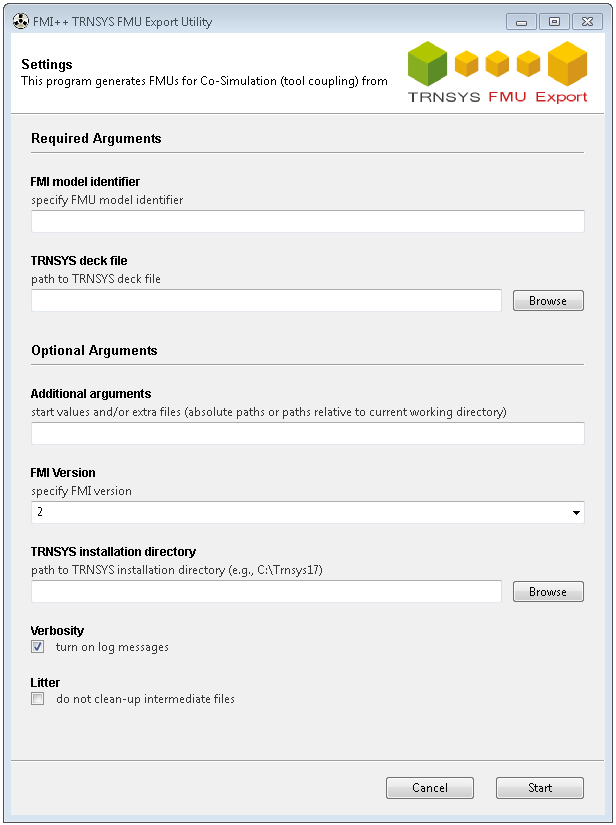
\includegraphics[width=0.98\textwidth]{trnsys_fmu_create_gui}}
\caption{The graphical user interface for creating an FMU.}
\label{fig:trnsys_fmu_create_gui}
\end{figure}

\clearpage

\section{Exporting an FMU using Python scripts}
\label{sec:export:command}

Instead of using the graphical user interface described in Chapter~\ref{sec:export:gui}, FMUs can also be generated using the \python script~\texttt{trnsys\_fmu\_create.py}, located in the installation directory.
The FMU is created by executing the script from the command prompt window (please refer to the \href{https://docs.python.org/2/faq/windows.html}{\python~FAQ} in case you need assistance with this).
Open the command prompt window, change to the directory containing the deck file and execute the script:
\begin{verbatim}
python <path_to_trnsys_fmu_dir>trnsys_fmu_create.py [-h] [-v] 
     -m <model_id> -d <deck_file> [-t <trnsys_install_dir>]
     [-f <fmi_version>] [<additional_file_1> ... <additional_file_N>]
     [var1=start_val1 ... varN=start_valN]
  \end{verbatim}
The path to the installation directory \verb!<path_to_trnsys_fmu_dir>! may be relative or absolute.
Optional arguments are enclosed by squared brackets \verb![!$\,$\ldots\verb!]!.

\textit{Mandatory input arguments}:
\begin{itemize}

  \item \verb!-m, --model-id!: Specify the FMU model identifier. \emph{Attention}: The FMU model identifier must fulfill the restrictions for C function names!
  \item \verb!-d, --deck-file!: Path to \trnsys deck file (absolute or relative).

\end{itemize}
\textit{Optional input arguments}:
\begin{itemize}

  \item \verb!-h, --help!: Display the help screen.
  \item \verb!-v, --verbose!: Turn on log messages.
  \item \verb!-l, --litter!: Do not clean-up intermediate files (e.g., log file with debug messages from Visual Studio compiler).
  \item \verb!-t, --trnsys-install-dir!: Absolute path to \trnsys installation directory. This should normally be set during the installation process (see Section~\ref{sec:install}).
  \item \verb!-f, --fmi-version!: Specify FMI version (\verb!1! or \verb!2!, default is \verb!2!)
  \item Additional files may be specified (e.g., weather data or input/output name lists) that will be automatically copied to the FMU. The specified files paths may be absolute or relative.
  \item Start values for variables may be defined. For instance, to set variable with name \verb!var1! to value 12.34, specify \verb!var1=12.34! in the command line as optional argument.

\end{itemize}
\chapter{Example}

\section{Overview}

This chapter provides a simple example of how to
\begin{itemize}
  \item include \type into a \trnsys model,
  \item export the model to an FMU and
  \item import the FMU into another application.
\end{itemize}

The example uses a simple thermal model that is exported as FMU.
The final FMU will have one input variable -- called \verb!control_signal! -- and three output variables -- called \verb!room_temperature!, \verb!mean_temperature! and \verb!value\_from\_file!.
The FMU will then be used as a plant model in a simple closed-loop control system implemented in \href{https://en.wikipedia.org/wiki/Dymola}{\dymola}.
Everything needed to reproduce the steps below can be found in the subfolder \texttt{examples} of the installation directory.

\begin{figure}[h!]
\centering{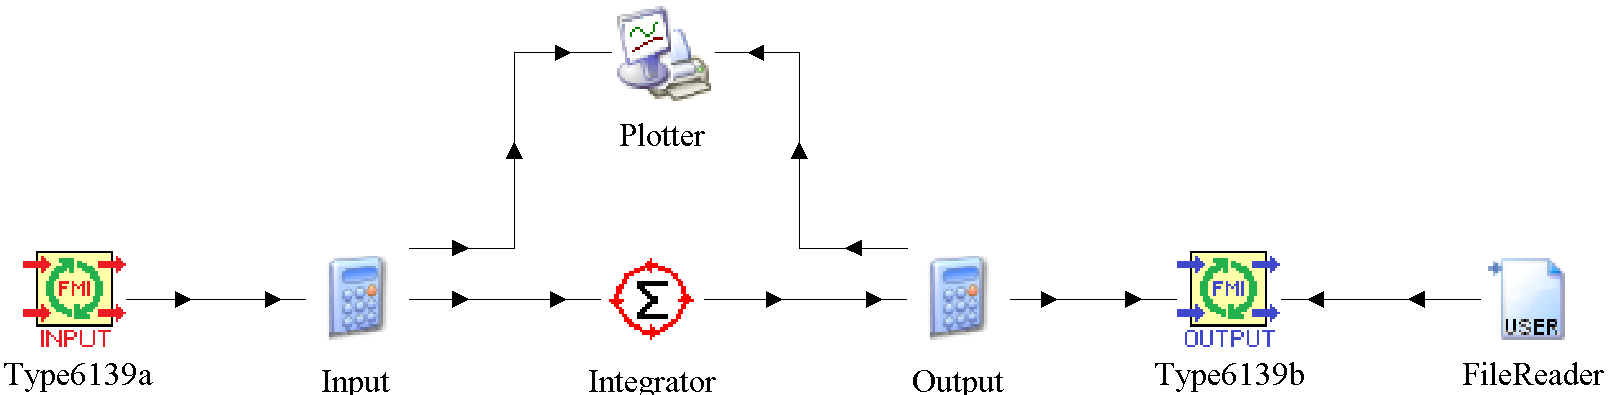
\includegraphics[width=\textwidth]{trnsys_model}}
\caption{Example \trnsys model.}
\label{fig:trnsys_model_example}
\end{figure}


\section{\trnsys model}

This example uses a very simple thermal room model that only consists of two equation blocks, an integrator block and a file reader, see Figure~\ref{fig:trnsys_model_example}.
The model is provided in file \verb!plant_room_model.tpf!, found in subfolder \verb!examples! of the installation directory.
In the following, the configuration of \typeb is explained step-by-step---the configuration for \typea is analogous.

For this example, the final FMU should have three output variables, called \texttt{room\_temperature}, \texttt{mean\_temperature} and \texttt{value\_from\_file}.
Within the \trnsys model, these \emph{FMU output variables} shall be represented by three \emph{\typeb input variables} called \texttt{room\_temperature\_output}, \texttt{mean\_temperature\_output} and \texttt{file\_output}.

To configure \typeb, proceed as follows (compare to Section~\ref{sec:export:model}):
\begin{itemize}
  \item Figure~\ref{fig:type_parameter_tab} shows the screen shot of the Proforma tab from Simulation Studio for \typeb.
  In this example, the corresponding FMU is supposed to have 3 outputs.
  Hence, the value for \texttt{number of FMI outputs} is set to~3.

  \item Consequently, the Input tab in Figure~\ref{fig:type_input_tab} shows 3 rows of type input variables.
  In this example they have been renamed from their default values to \texttt{room\_temperature\_output}, \texttt{mean\_temperature\_output} and \texttt{file\_output}.

  \item In the Special Cards tab, the third row specifies the FMU output variable names as a comma separated list, compare Figure~\ref{fig:type_special_cards_tab}.
  The names in this list will be matched sequentially with the input variable names specified in the Input tab.
  Hence, the numeric values associated with \typeb input variable \texttt{room\_temperature\_output} in the \trnsys model will be available via the FMU output variable \texttt{room\_temperature}, the value associated to \texttt{mean\_temperature\_output} will be available via \texttt{mean\_temperature} and the value associated to \texttt{file\_output} will be available via \texttt{value\_from\_file}.

  \item The input variables of \typeb are connected to the output variables of the \emph{Output} equation block in the usual way, see Figure~\ref{fig:type_connection}.

  \item To specify the simulation time and step size, either click the \textit{Control cards} icon in the side bar on the left or select from the menu bar on the top \textit{Assembly}~$\rightarrow$~\textit{Control cards}.
  For this example, set \textit{Simulation start time} to 0~hr, \textit{Simulation stop time} to 12~hr and \textit{Simulation time step} to 15~min.

  \item Finally, create the deck file by either clicking the \textit{Write input file} icon in the side bar on the left or select from the menu bar on the top \textit{Calculate}~$\rightarrow$~\textit{Create input file}.

\end{itemize}

\begin{figure}[h!]
\vspace*{5mm}
\centering{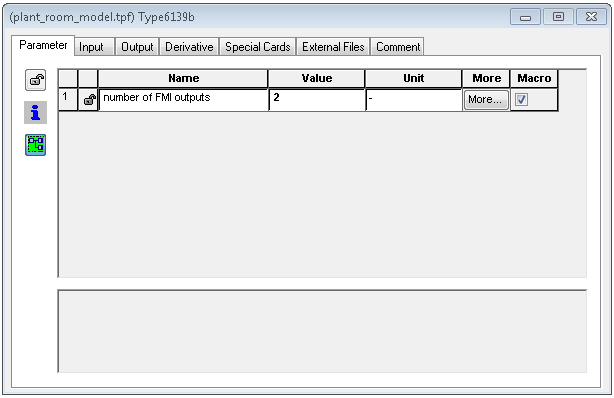
\includegraphics[width=0.95\textwidth]{type6139_parameter_tab}}
\caption{\typeb parameter tab.}
\label{fig:type_parameter_tab}
\end{figure}

\begin{figure}[h!]
\centering{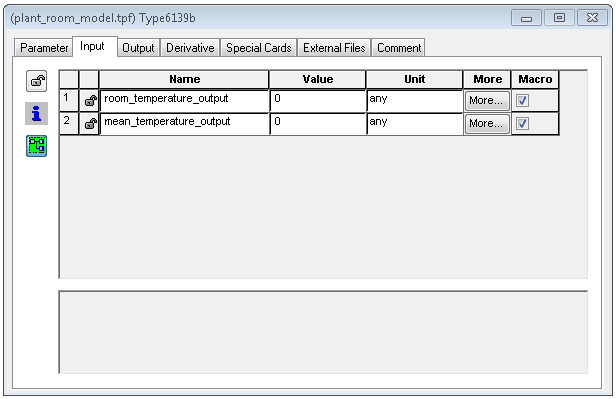
\includegraphics[width=0.95\textwidth]{type6139_input_tab}}
\caption{\typeb input tab.}
\label{fig:type_input_tab}
\end{figure}


\begin{figure}[h!]
\centering{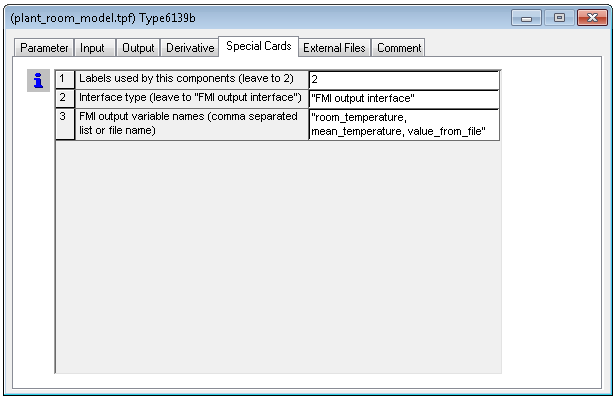
\includegraphics[width=0.95\textwidth]{type6139_special_cards_tab}}
\caption{\typeb special cards tab.}
\label{fig:type_special_cards_tab}
\end{figure}

\begin{figure}[h!]
\vspace*{5mm}\centering{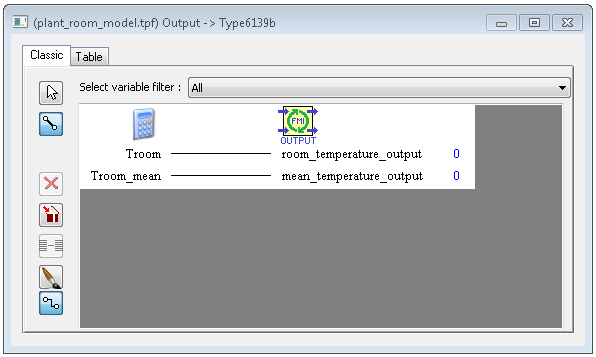
\includegraphics[width=0.95\textwidth]{type6139b_connection}}
\vspace*{5mm}\centering{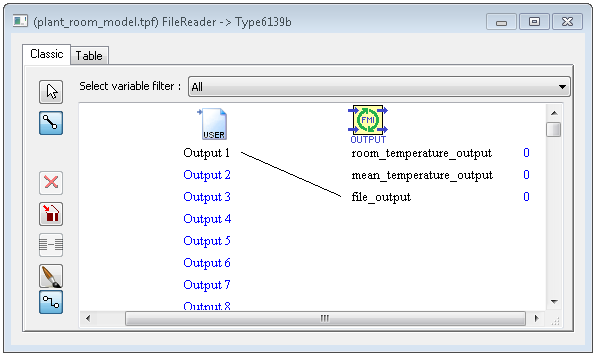
\includegraphics[width=0.95\textwidth]{type6139b_connection2}}
\caption{The inputs of \typeb are connected to the output variables of the \emph{Output} equation block and \emph{FileReader} file reader block.}
\label{fig:type_connection}
\end{figure}


\begin{figure}[h!]
\centering{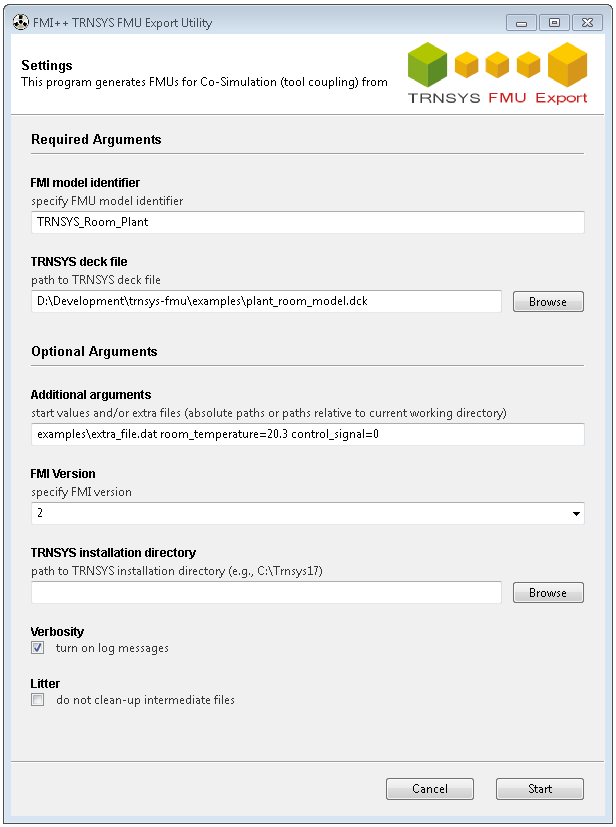
\includegraphics[width=0.95\textwidth]{trnsys_fmu_create_example_gui}}
\caption{Inputs to the graphical user interface.}
\label{fig:trnsys_fmu_create_example_gui}
\end{figure}

\begin{figure}[h!]
\centering{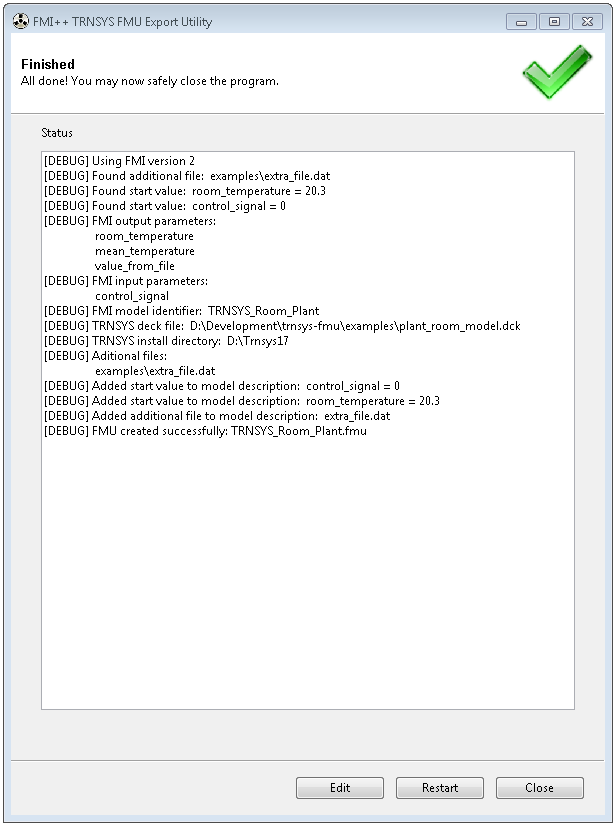
\includegraphics[width=0.95\textwidth]{trnsys_fmu_create_example_result}}
\caption{Output message from the graphical user interface.}
\label{fig:trnsys_fmu_create_example_result}
\end{figure}

\clearpage

\section{Generating the FMU}

\subsection{Graphical user interface}

Start program \texttt{trnsys\_fmu\_create.exe} in the installation directory by double-clicking it.
Then provide the following inputs (see Figure~\ref{fig:trnsys_fmu_create_example_gui}):
\begin{itemize}

  \item FMI model identifier: \textit{TRNSYS\_Room\_Plant}

  \item TRNSYS deck file: click \texttt{Browse} and select file \textit{plant\_room\_model.dck} from the examples folder

  \item Additional arguments: \textit{examples{\textbackslash}extra\_file.dat room\_temperature=20.3 control\_signal=0}. 
  (Note the the path of the extra file relative to the installation directory.)

\end{itemize}
Then click the \texttt{Start} button to create the FMU.


Some comments:
\begin{itemize}

  \item The model is exported with the FMI model identifier \verb!TRNSYS_Room_Plant!.
  Hence, the FMU created will be named \verb!TRNSYS_Room_Plant.fmu!.

  \item The command specifies several start values of FMI input/output variables in the additional arguments (\verb!control_signal=0! and \verb!room_temperature=20.3!), compare to the results in Section~\ref{sec:example:results}.
  
  \item The verbosity check box is by default selected, which  causes the script to output additional information.
  In case the scripts executes successfully, this should produce the outputs shown in Figure~\ref{fig:trnsys_fmu_create_example_result}.

\end{itemize}


\subsection{Running the \python script}

Instead of using the graphical user interface, the FMU can be generated with the help of the \python script explained in Section~\ref{sec:export:command}.
For this example, the following command has to be issued in the command prompt window from the \texttt{examples} directory:
\begin{verbatim}
python.exe ..\trnsys_fmu_create.py -v -m TRNSYS_Room_Plant
      -d plant_room_model.dck extra_file.dat
      room_temperature=20.3 control_signal=0
\end{verbatim}
\textbf{Attention}:
The full command is too long to be displayed in one line in this document, hence above it is split in two lines.
In the command prompt window, the command has to be written as one uninterrupted string (i.e.,~without carriage returns \keys{\return} in between).

Some comments:
\begin{itemize}
  \item The model is exported with the FMI model identifier \verb!TRNSYS_Room_Plant!, according to the value supplied to the mandatory input argument \verb!-m!.
  Hence, the FMU created will be named \verb!TRNSYS_Room_Plant.fmu!.

  \item The command specifies several start values of FMI input/output variables in the additional arguments (\verb!control_signal=0! and \verb!room_temperature=20.3!), compare to the results in Section~\ref{sec:example:results}.
  
  \item The optional argument \verb!-v! causes the script to output additional information. In case the scripts executes successfully, the output should look similar to the following:
\begin{verbatim}
[DEBUG] Using FMI version 2
[DEBUG] Found additional file:  extra_file.dat
[DEBUG] Found start value:  room_temperature = 20.3
[DEBUG] Found start value:  control_signal = 0
[DEBUG] FMI output parameters:
         room_temperature
         mean_temperature
         value_from_file
[DEBUG] FMI input parameters:
         control_signal
[DEBUG] FMI model identifier:  TRNSYS_Room_Plant
[DEBUG] TRNSYS deck file:  examples\plant_room_model.dck
[DEBUG] TRNSYS install directory:  D:\Trnsys17
[DEBUG] Aditional files:
         extra_file.dat
[DEBUG] Added start value to model description:  control_signal = 0
[DEBUG] Added start value to model description:  room_temperature = 20.3
[DEBUG] Added additional file to model description:  extra_file.dat
[DEBUG] FMU created successfully: TRNSYS_Room_Plant.fmu
\end{verbatim}

\end{itemize}


\subsection{Checking the content}

\textbf{Note}: After successfully generating the FMU it is in general not necessary to check the content of the resulting FMU manually.
This section only intends to give some background information and can be skipped when working through the example.

Successfully running the script creates the FMU, i.e., a file called \verb!TRNSYS_Room_Plant.fmu!.
Since FMUs are just ZIP files, one can use standard ZIP archive processing tools (such as \href{http://www.7-zip.org/}{7-Zip}) to inspect them.
The contents of \verb!TRNSYS_Room_Plant.fmu! are as follows:
\begin{itemize}
  \item \verb!binaries!: This folder contains the shared library \verb!TRNSYS_Room_Plant.dll! in a subfolder called \verb!win32!.
  This shared library implements the coupling to \trnsys at runtime.

  \item \verb!resources!: This folder contains the deck file \verb!plant_room_model.dck! and the additional file \verb!extra_file.dat!. Both files will be loaded at runtime.

  \item \verb!modelDescription.xml!: This is an XML-based description of the model contained by the FMU.

\end{itemize}

The XML-based model description contains all relevant information about the model contained in the FMU:
\begin{itemize}
  \item the FMI model identifier and other model meta data, see attributes of XML node \texttt{fmiModelDescription}

  \item the input and output variables of the model, listed as separate \texttt{ScalarVariable} nodes

  \item information about the functionality supported by the simulation tool, see XML node \verb!CoSimulation!
  
  \item information about how to run the model with the specified simultion tool, see XML node \verb!VendorAnnotations.Tool!
\end{itemize}

For the given example, the XML model description should be very similar to the following:
\begin{verbatim}
<?xml version="1.0" encoding="UTF-8"?>
<fmiModelDescription
  xmlns:xsi="http://www.w3.org/2001/XMLSchema-instance"
  fmiVersion="2.0"
  modelName="plant_room_model"
  guid="{dde75d48-d134-11e7-9d0f-f365722dd787}"
  generationTool="FMI++ TRNSYS Export Utility"
  author="user"
  generationDateAndTime="2017-11-24T17:31:04"
  variableNamingConvention="flat"
  numberOfEventIndicators="0">
  <CoSimulation
    modelIdentifier="TRNSYS_Room_Plant"
    needsExecutionTool="false"
    canHandleVariableCommunicationStepSize="false"
    canNotUseMemoryManagementFunctions="true"
    canInterpolateInputs="false"
    maxOutputDerivativeOrder="0"
    canGetAndSetFMUstate="false"
    providesDirectionalDerivative="false"/>
  <VendorAnnotations>
    <Tool name="FMI++Export">
      <Executable
        executableURI="file:///D:/Trnsys17/exe/trnexe.exe"
        entryPointURI="fmu://resources/plant_room_model.dck"
        preArguments=""
        postArguments="/n"/>
      <File file="fmu://resources/extra_file.dat"/>
    </Tool>
  </VendorAnnotations>
  <ModelVariables>
    <ScalarVariable name="control_signal"
	  valueReference="1"
	  variability="continuous"
	  causality="input" >
      <Real start="0"/>
    </ScalarVariable>
    <ScalarVariable name="room_temperature"
	  valueReference="1001" 
	  variability="continuous" 
	  causality="output" 
	  initial="exact">
      <Real start="20.3"/>
    </ScalarVariable>
    <ScalarVariable name="mean_temperature" 
	  valueReference="1002" 
	  variability="continuous" 
	  causality="output" >
      <Real/>
    </ScalarVariable>
    <ScalarVariable name="value_from_file"
	  valueReference="1003" 
	  variability="continuous" 
	  causality="output" >
      <Real/>
    </ScalarVariable>
  </ModelVariables>
  <ModelStructure/>
</fmiModelDescription>
\end{verbatim}

\section{Using the FMU}

\subsection{\dymola model}

Subfolder \verb!examples! of the installation directory also contains a \dymola model that can be used to test the created \trnsys FMU, called \verb!trnsys_closed_loop_control_example.mo!.


This model implements a simple closed-loop control system that uses the FMU as black-box plant model, see Figure~\ref{fig:dymola_example}.
Depending on the room temperature---provided by FMU output variable \verb!room_temperature!---the controller turns the room's heating on or off---by setting the FMU input variable \verb!control_signal! to either 0~or~1.
More precisely, the model implements a hysteresis controller that turns the heater on as soon as the room temperature falls below 20.5$\,^\circ$C and turns it off when it exceeds 21.5$\,^\circ$C.

\begin{figure}[h!]
\centering{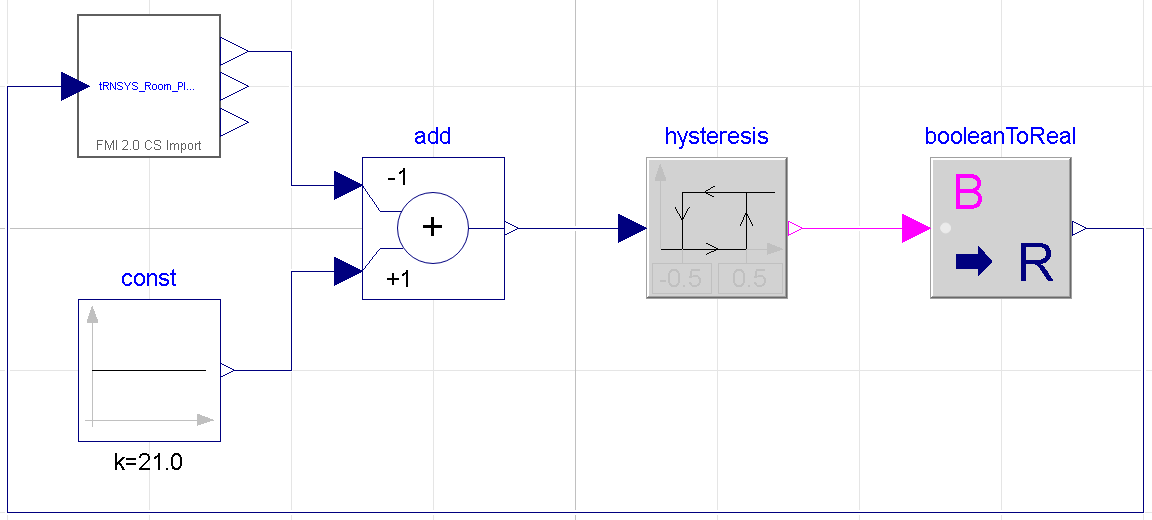
\includegraphics[width=0.99\textwidth]{dymola_example}}
\caption{\dymola example.}
\label{fig:dymola_example}
\end{figure}

To run the model, start \dymola~2018 (32-bit version), import the FMU and load the \dymola model. \textbf{Note}: Please check the \dymola documentation on how to import an FMU for Co-Simulation.


\subsection{Results}
\label{sec:example:results}

Figure~\ref{fig:dymola_output} shows the results of the simulated \dymola model.
Depicted is the room temperature as computed by \trnsys, which is kept within 21.0$\,^\circ$C~$\pm$0.5$\,^\circ$C by the \dymola controller.
Please note that the start value of the room temperature is 20.3$\,^\circ$C, as specified at the creation of the FMU.

\begin{figure}[h!]
\centering{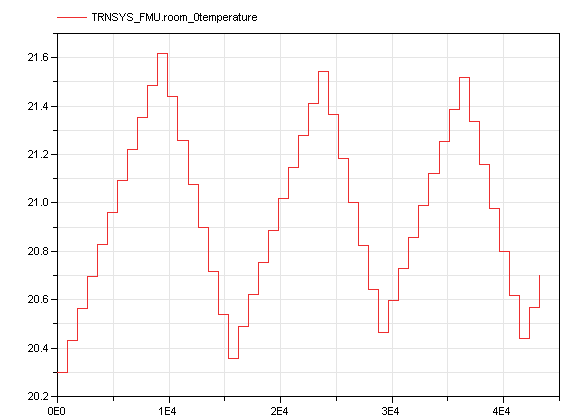
\includegraphics[width=0.99\textwidth]{dymola_output}}
\caption{Example \dymola output.}
\label{fig:dymola_output}
\end{figure}

Due to the fixed simulation step size of 15 minutes, the switching of the controller state does not happen at the exact edges of the controller's dead-band (i.e., at 20.5$\,^\circ$C and 21.5$\,^\circ$C).
Please be aware that this is not a shortcoming of the FMU itself, but due to \trnsys's restriction to fixed simulation time steps.
Such simulation artifacts are unavoidable in fixed-step co-simulation and have to be taken into account by the modeler (e.g., by choosing an adequate simulation step size).

\chapter{Troubleshooting}

In case the created FMU does not work as expected, the best way to check what happened is to take a look into the log file created by \trnsys.
This file is written in the unzipped folder of the FMU, called \texttt{<deck-file>.log}, where \texttt{<deck-file>} corresponds to the deck file name included in the FMU.
Please note, the location of this unzipped folder depends on the co-simulation environment used to access the FMU.

\chapter{Appendix}

\section{The \fmipp \trnsys Export Utility License}
\label{trnsys_fmu_license}

Copyright (c) 2015, AIT Austrian Institute of Technology GmbH. All
rights reserved.

Redistribution and use in source and binary forms, with or without
modification, are permitted provided that the following conditions are
met:

\begin{itemize}
\itemsep1pt\parskip0pt\parsep0pt
\item
  Redistributions of source code must retain the above copyright notice,
  this list of conditions and the following disclaimer.
\item
  Redistributions in binary form must reproduce the above copyright
  notice, this list of conditions and the following disclaimer in the
  documentation and/or other materials provided with the distribution.
\end{itemize}

THIS SOFTWARE IS PROVIDED BY THE COPYRIGHT HOLDERS AND CONTRIBUTORS ``AS
IS'' AND ANY EXPRESS OR IMPLIED WARRANTIES, INCLUDING, BUT NOT LIMITED
TO, THE IMPLIED WARRANTIES OF MERCHANTABILITY AND FITNESS FOR A
PARTICULAR PURPOSE ARE DISCLAIMED. IN NO EVENT SHALL THE COPYRIGHT
HOLDER OR CONTRIBUTORS BE LIABLE FOR ANY DIRECT, INDIRECT, INCIDENTAL,
SPECIAL, EXEMPLARY, OR CONSEQUENTIAL DAMAGES (INCLUDING, BUT NOT LIMITED
TO, PROCUREMENT OF SUBSTITUTE GOODS OR SERVICES; LOSS OF USE, DATA, OR
PROFITS; OR BUSINESS INTERRUPTION) HOWEVER CAUSED AND ON ANY THEORY OF
LIABILITY, WHETHER IN CONTRACT, STRICT LIABILITY, OR TORT (INCLUDING
NEGLIGENCE OR OTHERWISE) ARISING IN ANY WAY OUT OF THE USE OF THIS
SOFTWARE, EVEN IF ADVISED OF THE POSSIBILITY OF SUCH DAMAGE.


\section{The \fmipp License}
\label{fmipp_license}

Copyright (c) 2013, AIT Austrian Institute of Technology GmbH. All
rights reserved.

Redistribution and use in source and binary forms, with or without
modification, are permitted provided that the following conditions are
met:

\begin{itemize}
\itemsep1pt\parskip0pt\parsep0pt
\item
  Redistributions of source code must retain the above copyright notice,
  this list of conditions and the following disclaimer.
\item
  Redistributions in binary form must reproduce the above copyright
  notice, this list of conditions and the following disclaimer in the
  documentation and/or other materials provided with the distribution.
\end{itemize}

THIS SOFTWARE IS PROVIDED BY THE COPYRIGHT HOLDERS AND CONTRIBUTORS ``AS
IS'' AND ANY EXPRESS OR IMPLIED WARRANTIES, INCLUDING, BUT NOT LIMITED
TO, THE IMPLIED WARRANTIES OF MERCHANTABILITY AND FITNESS FOR A
PARTICULAR PURPOSE ARE DISCLAIMED. IN NO EVENT SHALL THE COPYRIGHT
HOLDER OR CONTRIBUTORS BE LIABLE FOR ANY DIRECT, INDIRECT, INCIDENTAL,
SPECIAL, EXEMPLARY, OR CONSEQUENTIAL DAMAGES (INCLUDING, BUT NOT LIMITED
TO, PROCUREMENT OF SUBSTITUTE GOODS OR SERVICES; LOSS OF USE, DATA, OR
PROFITS; OR BUSINESS INTERRUPTION) HOWEVER CAUSED AND ON ANY THEORY OF
LIABILITY, WHETHER IN CONTRACT, STRICT LIABILITY, OR TORT (INCLUDING
NEGLIGENCE OR OTHERWISE) ARISING IN ANY WAY OUT OF THE USE OF THIS
SOFTWARE, EVEN IF ADVISED OF THE POSSIBILITY OF SUCH DAMAGE.

\section{The \boost Software License}
\label{boost_license}

Version 1.0 - August 17th, 2003

Permission is hereby granted, free of charge, to any person or organization
obtaining a copy of the software and accompanying documentation covered by
this license (the "Software") to use, reproduce, display, distribute,
execute, and transmit the Software, and to prepare derivative works of the
Software, and to permit third-parties to whom the Software is furnished to
do so, all subject to the following:

The copyright notices in the Software and this entire statement, including
the above license grant, this restriction and the following disclaimer,
must be included in all copies of the Software, in whole or in part, and
all derivative works of the Software, unless such copies or derivative
works are solely in the form of machine-executable object code generated by
a source language processor.

THE SOFTWARE IS PROVIDED "AS IS", WITHOUT WARRANTY OF ANY KIND, EXPRESS OR
IMPLIED, INCLUDING BUT NOT LIMITED TO THE WARRANTIES OF MERCHANTABILITY,
FITNESS FOR A PARTICULAR PURPOSE, TITLE AND NON-INFRINGEMENT. IN NO EVENT
SHALL THE COPYRIGHT HOLDERS OR ANYONE DISTRIBUTING THE SOFTWARE BE LIABLE
FOR ANY DAMAGES OR OTHER LIABILITY, WHETHER IN CONTRACT, TORT OR OTHERWISE,
ARISING FROM, OUT OF OR IN CONNECTION WITH THE SOFTWARE OR THE USE OR OTHER
DEALINGS IN THE SOFTWARE.

\section{Version History}

\begin{itemize}
  \item v0.1: first release version
  \item v0.2: added documentation, minor code clean-up
  \item v0.3: allow same deck file name and FMU model identifier, renamed Python scripts, code clean-up in Python scripts, allow running Python script for creating an FMU from arbitrary directory, add section on troubleshooting to documentation
  \item v0.4: updated documentation
  \item v0.5: support installation paths containing spaces (e.g., \texttt{C:\symbol{92}Program Files\symbol{92}trnsys-fmu}).
  \item v0.6: allow definition of FMU input/output names via files containing lists
\end{itemize}



%----------------------------------------------------------------------------------------
%	INDEX
%----------------------------------------------------------------------------------------

%\cleardoublepage
%\phantomsection
%\setlength{\columnsep}{0.75cm}
%\addcontentsline{toc}{chapter}{\textcolor{ocre}{Index}}
%\printindex

%----------------------------------------------------------------------------------------

\end{document}
